\documentclass[a4paper, 12pt]{article} % Adicionado tamanho do papel e fonte maior (12pt)
\usepackage[utf8]{inputenc}
\usepackage{array}
% --- Configurações de Margem ---
\usepackage[a4paper, margin=2.5cm]{geometry} % É AQUI QUE A MÁGICA ACONTECE! 
% Se o professor exigir ABNT, troque a linha acima por:
% \usepackage[a4paper, left=3cm, right=2cm, top=3cm, bottom=2cm]{geometry}
\usepackage{float}
% --- Idioma e Codificação ---
\usepackage[T1]{fontenc}
\usepackage[utf8]{inputenc} % Garante que acentos funcionem (opcional nas versões mais recentes, mas seguro)
\usepackage[portuguese]{babel} % Hifenização correta e tradução (ex: "Abstract" vira "Resumo")
\usepackage{tabularx}
% --- Pacotes Úteis para Relatórios ---
\usepackage{graphicx} % Para inserção de imagens (o que você já tinha)
\usepackage{hyperref} % Deixa o sumário e as URLs clicáveis
\usepackage{url}
\usepackage{microtype} % Melhora drasticamente a justificação do texto (evita buracos brancos)
\usepackage{indentfirst} % Indenta o primeiro parágrafo de cada seção (padrão do português)
\usepackage[backend=biber, style=abnt]{biblatex} % style=abnt para ABNT, ou style=ieee
\addbibresource{lib.bib}
\usepackage{listings}
\usepackage{xcolor}

% Configuração básica para parecer com o seu exemplo
\lstset{
  basicstyle=\ttfamily\small,
  backgroundcolor=\color{gray!10},
  frame=single,
  breaklines=true
}

% --- Dados da Capa ---
\title{\textbf{EP2 de Bancos de dados}}
\author{\small\textit{ Enzo Furegatti Spinella -- 14568198}}


\newcommand{\code}[1]{\texttt{#1}}
\begin{document}

\maketitle

% Certifique-se de que os seguintes pacotes estejam no preâmbulo do seu documento (antes do \begin{document}):
% \usepackage{graphicx}
% \usepackage{amsmath}
% \usepackage{booktabs}
% \usepackage{float}

\section{Metodologia}
\label{sec:metodologia}

Para avaliar as soluções de indexação vetorial discutidas teoricamente, foi conduzido um experimento prático e controlado comparando o desempenho da extensão \textit{pgvector} (PostgreSQL) com o banco de dados nativo vetorial Qdrant. A metodologia adotada consistiu na execução de testes de estresse automatizados, visando mensurar três eixos principais: tempo de indexação, latência de consulta e precisão da busca aproximada.

\subsection{Ambiente de Execução}
A fim de garantir a isonomia e a reprodutibilidade do experimento, ambas as ferramentas foram executadas sob restrições idênticas em um ambiente isolado utilizando contêineres Docker. Os testes foram realizados em uma máquina equipada com o sistema operacional Pop!\_OS, processador Intel Core i7-9750H e 16GB de memória RAM.

Para a comunicação com os bancos de dados, desenvolveu-se um \textit{script} em Python. A conexão com o PostgreSQL foi estabelecida via \textit{socket} persistente utilizando a biblioteca \texttt{psycopg2}, enquanto o Qdrant foi acessado por meio de seu cliente oficial, que opera sobre o protocolo HTTP/REST.

Para garantir a reprodutibilidade integral deste estudo empírico, o código-fonte em Python desenvolvido para a automação e coleta de métricas do experimento, bem como os arquivos de configuração de infraestrutura dos contêineres (\textit{docker-compose}), foram disponibilizados publicamente. O repositório contém as instruções detalhadas de configuração do ambiente e execução do referencial de testes

O repositório completo pode ser acessado em: \url{https://github.com/SQL-2026-Trabalho/ep2}

\subsection{Conjunto de Dados e Geração de Embeddings}
O \textit{dataset} utilizado para popular as bases de dados foi um subconjunto de 5.000 amostras textuais extraídas do repositório público \texttt{dair-ai/emotion}. A conversão do texto bruto para representações vetoriais (\textit{embeddings}) foi realizada \textit{offline} utilizando a biblioteca \texttt{sentence-transformers}, por meio do modelo pré-treinado \texttt{all-MiniLM-L6-v2}. 

Este modelo foi selecionado por seu excelente balanço entre velocidade e qualidade semântica, gerando vetores densos de 384 dimensões. Do conjunto total, 4.900 documentos foram destinados à inserção nos bancos de dados, enquanto os 100 vetores restantes foram isolados para atuar exclusivamente como parâmetros de consulta (\textit{queries}).

\subsection{Desenho do Experimento e Métricas}
Para mitigar flutuações de desempenho causadas pelo escalonador do sistema operacional ou por \textit{cache misses}, o experimento foi desenhado para executar 30 iterações independentes ($n=30$). Em cada rodada, os índices foram integralmente recriados. As seguintes métricas foram coletadas:

\begin{itemize}
    \item \textbf{Tempo de Inserção e Indexação:} Tempo total (em segundos) necessário para gravar os 4.900 vetores e construir os índices de busca aproximada (HNSW em ambas as ferramentas).
    \item \textbf{Latência de Consulta:} Tempo médio (em milissegundos) para retornar os 10 vizinhos mais próximos ($k=10$) para o lote de 100 \textit{queries}.
    \item \textbf{Recall@10:} Métrica de precisão calculada pela intersecção entre os resultados da busca aproximada e um "gabarito" exato. O gabarito foi gerado forçando o PostgreSQL a realizar uma varredura sequencial ($O(N)$) utilizando a métrica de similaridade de cosseno.
\end{itemize}

% ---------------------------------------------------------

\section{Resultados e Avaliação Experimental}
\label{sec:result}

Os dados brutos coletados nas 30 iterações foram consolidados, permitindo a extração da média ($\mu$) e do desvio padrão ($\sigma$) para cada ferramenta, conferindo validade estatística à comparação.

\subsection{Desempenho de Indexação}
A Figura \ref{fig:insercao} ilustra o tempo médio exigido por cada sistema para realizar o \textit{bulk insert} dos vetores e estruturar o grafo do índice HNSW[cite: 2].

\begin{figure}[H]
    \centering
    % Substitua pela escala ideal se a imagem ficar muito grande
    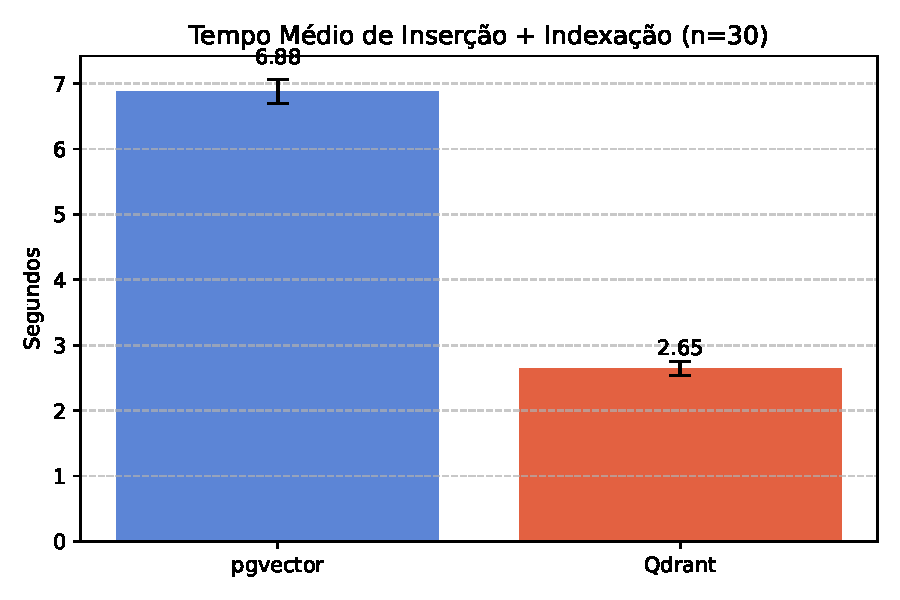
\includegraphics[width=0.7\textwidth]{grafico_insercao.pdf}
    \caption{Comparativo do tempo médio de inserção e construção do índice HNSW ($n=30$). As barras de erro indicam o desvio padrão observado[cite: 2].}
    \label{fig:insercao}
\end{figure}

O Qdrant apresentou uma vantagem expressiva nesta etapa, concluindo o processo em uma média de 2,65 segundos, contra os 6,88 segundos demandados pelo \textit{pgvector}[cite: 2]. Este resultado evidencia a otimização arquitetural do Qdrant para o processamento nativo em lotes (\textit{batches}). A extensão do PostgreSQL, por herdar o motor relacional padrão focado em transações ACID individuais, impõe um \textit{overhead} maior durante operações massivas de escrita vetorial.

\subsection{Latência e Precisão de Consulta}
No que tange ao tempo de resposta para recuperação de informação, o cenário se inverteu, conforme demonstrado na Figura \ref{fig:latencia}[cite: 3].

\begin{figure}[H]
    \centering
    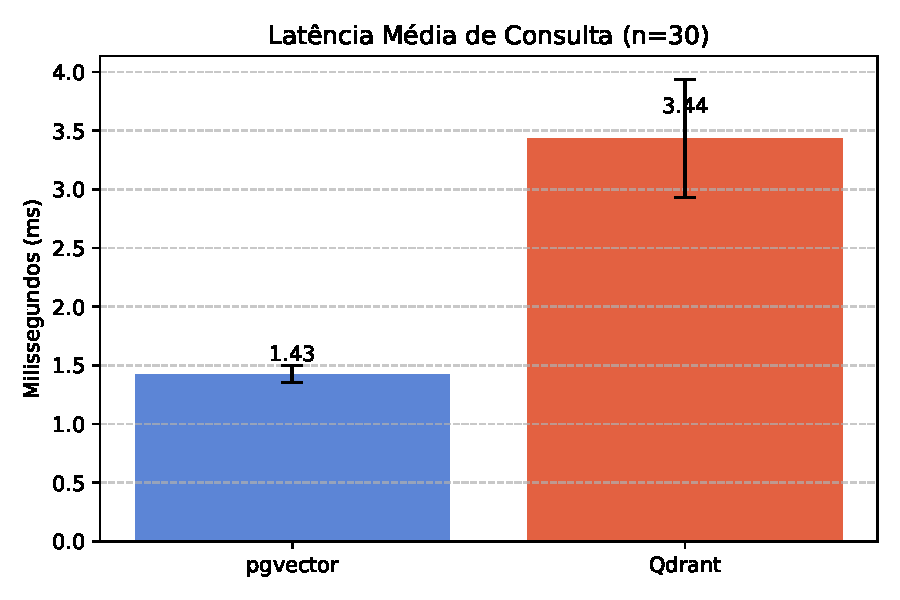
\includegraphics[width=0.7\textwidth]{grafico_latencia.pdf}
    \caption{Comparativo da latência média por consulta ($k=10$). As barras de erro evidenciam a maior variância na comunicação com o Qdrant[cite: 3].}
    \label{fig:latencia}
\end{figure}

O \textit{pgvector} obteve uma latência substancialmente menor, registrando uma média de 1,43 ms por consulta, em contraste com os 3,44 ms observados no Qdrant[cite: 3]. Destaca-se na Figura \ref{fig:latencia} a considerável margem de erro ($\sigma$) atrelada ao Qdrant[cite: 3]. Esta variância superior e a maior latência média são explicadas, no contexto deste \textit{dataset} de menor escala (4.900 registros), pelo custo inerente de rede. Enquanto o acesso ao Qdrant exige o estabelecimento e a resolução de requisições HTTP, o PostgreSQL beneficia-se de conexões binárias persistentes e mais próximas do \textit{kernel}. Em volumes de dados que não excedem a memória principal, o \textit{overhead} de comunicação do cliente REST ofusca a velocidade de busca interna da \textit{engine} em Rust.

Por fim, a avaliação qualitativa da recuperação demonstrou que ambas as implementações do algoritmo HNSW são altamente confiáveis. Ao comparar os identificadores retornados contra o gabarito de busca exaustiva, o \textit{pgvector} atingiu um \textit{Recall@10} médio de 98.42\%, enquanto o Qdrant registrou 100.00\%. Esses índices confirmam que a aceleração obtida pela aproximação do índice não compromete de forma estatisticamente significativa a corretude semântica dos resultados.

\end{document}

\printbibliography
\end{document}
